\chapter{Introduction}
The space we exist in is three dimensional, and this pervades every aspect of our interaction with reality. Everything we touch, see, and hear behaves according to the rules of this three dimensional space and this has made humans exceptionally proficient at reasoning about it, navigating through it, and modelling the behaviour of things within it. Yet when we interact with our computers, an increasingly important part of our everyday lives, most of us do so exclusively through two dimensional user interfaces. 
 
\section{Two Dimensional User Interfaces}

The two dimensional space in which we interact with computers has come to define these interactions in the same way that the three dimensional space in which we exist defines our interaction with reality. We use our fingers or a mouse press 2D buttons and open 2D menus, driving change in the application's 2D interfaces which the windowing system composites into a 2D image to be sent to a 2D display. While this is natural for some intrinsically 2D concepts, like documents and images, other concepts which have no intrinsic spatial embedding, like file systems and networks, are also embedded in 2D when they are presented to the user in order to allow users to reason about them spatially. Even in applications which are intrinsically 3D, like physical simulation and modelling tools, the 3D application space is disjoint from the space in which the user exists (by necessity, since the application has no knowledge of the 3D relationship between the display and the user) and interaction between the 3D application space and the 3D user is traditionally done with 2D input events and 2D images.  

\begin{figure}[ht!]
\centering
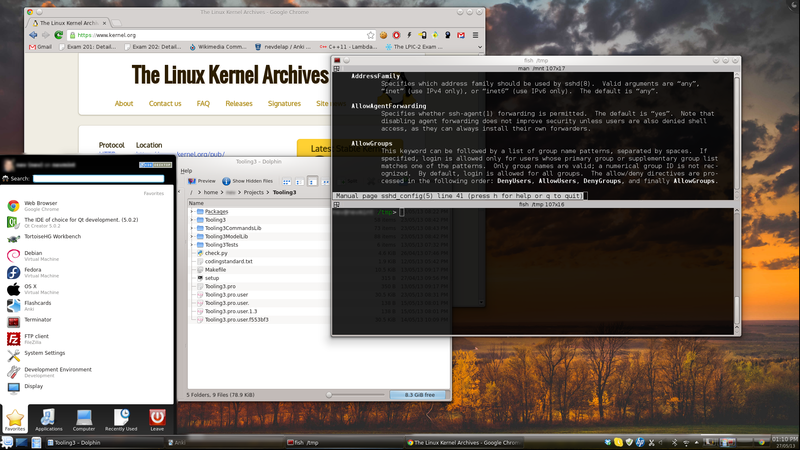
\includegraphics[width=1.0\textwidth]{images/kde.png}
\caption{An example of a typical 2D user interface, showing windows and the desktop environment on a Linux system. Image taken from  \protect\cite{kde-image}}
\label{fig:kde}
\end{figure}
	
The flat nature of contemporary graphical user interfaces has come to define not just the way we interact with applications, but has also become an important factor in the physical design of the computers that run these applications. This is particularly apparent in the mobile computer space, where cost, weight, display power, and mobility concerns push devices toward ever smaller physical profiles, while usability concerns drive the devices toward larger interface surfaces, leading the profile of mobile computers to become flattened against their displays, with the devices acting as a physical embedding of the 2D computer interface within the 3D space in which the computer exists. This forces users to make a tradeoff between the physical profile of their device and the usable size of their interface; larger displays drive up mass both directly and through the need for a larger battery to meet increased power demands, but a smaller displays limit the usable size of the human-computer interface which limits the usability of the device. In desktop computers the same tradeoff must be made, because even absent power and weight concerns the size of the interface is still constrained by the cost of the displays and the physical space needed to mount them in view of the user.

Two dimensional user interfaces are certainly not all bad. There is a natural analog between interacting with documents, images, and folders on a desk and interacting with their digital counterparts on a 2D display (which forms the underpinnings of the familiar desktop metaphor). 2D interfaces also map well onto commercially available display hardware as a result of the two co-evolving for several decades, which keeps the hardware cost of 2D interfaces relatively low. 2D interfaces are mature and well studied, and there is a rich software ecosystem surrounding them which includes sophisticated, full featured user interface toolkits and advanced windowing systems, as well as a broad set of end user applications that provide 2D graphical frontends for almost every task a user need perform on a computer. Users are also familiar with the operation of 2D interfaces, which greatly reduces the time needed for users to learn new applications and improves their productivity with existing applications. 

There are certain applications, like document and photo editing and command line interaction, which fit well with 2D interfaces, and in these applications moving away from 2D interactions would likely be detrimental. However, many applications are intrinsically 3D, or are not intrinsically spatial at all and are embedded in a 2D space because it is simple and well supported, and a transition to 3D interaction has the potential to greatly improve  the usability of such applications \cite{bowman_theory_practice}.

\section{Three Dimensional User Interfaces}

\begin{figure}[ht!]
\centering
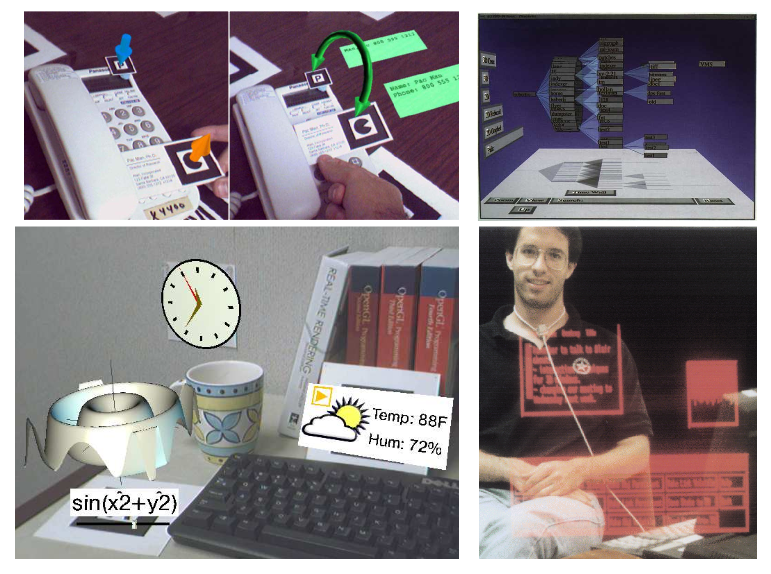
\includegraphics[width=1.0\textwidth]{images/3dui-examples.png}
\caption{Examples of 3D user interfaces. On the left is ARWin \protect\cite{arwin}, on the top right is an example file browser from \protect\cite{info-vis}, on the bottom right is Windows on the World \protect\cite{wotw}}
\label{fig:3dui-example}
\end{figure}

The hardware, software, and theory surrounding high quality 3D human-computer interaction has been the subject of academic research for many decades, and the improved spatial reasoning this provides has been demonstrated to improve usability in a  number of applications  \cite{bowman_theory_practice}. 3D user interfaces are a broad group of interaction paradigms, including everything from desktop 3D modeling with a mouse and keyboard to fully immersive virtual reality.  This thesis focuses on ‘immersive' 3D interfaces, which is used here to refer to 3D interfaces in which the user perceives the 3D interface elements to be in the same 3D space as their body, and has some way of manipulating these interface elements in 3D with corresponding 3D motion by some part of their body.  The hardware needed to support these types of interfaces has traditionally been very expensive, but recent technological improvements in a number of fields have brought many of the core hardware technologies onto the consumer market, bringing both high quality 3D input devices and immersive 3D displays into the reach of everyday computer users.

\subsection{Three Dimensional Input Devices}

Early 3D input devices to come into the consumer 3D interaction market were largely marketed as video game accessories, though their availability has led to their use in a wide variety of other application. These devices can be broadly categorized into two groups: devices which resolve the position and/or orientation of an element held or worn by the user, and range-imaging cameras, which produce a 3D image of a passive scene which contains no sensing elements itself.

\begin{figure}[ht!]
\centering
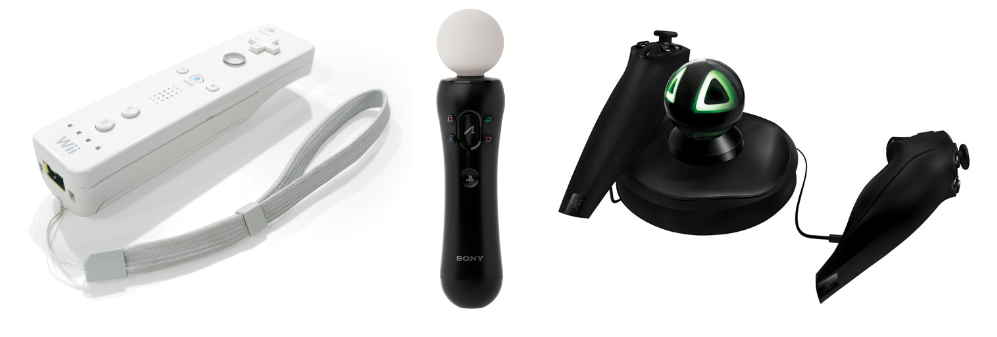
\includegraphics[width=1.0\textwidth]{images/motion-controllers.png}
\caption{From left to right the Wiimote, Playstation Move, and Razer Hydra. Images taken from \protect\cite{wiimote-image}, \protect\cite{ps-move-image}, and \protect\cite{hydra-image}, respectively.}
\label{fig:motion-controllers}
\end{figure}

The first category had its first commercial success in consumer markets in 2006, when Nintendo introduced the Wii Remote, or `Wiimote', as the primary controller for its new Wii entertainment system. This controller, unlike traditional game console controllers, was able to sense its position, orientation, and acceleration along 3 axes. The Wiimote provided limited 3D control within Wii games, and was soon adopted by developers for a wider variety of tasks, including controlling the visualization of volumetric medical data \cite{wiimote-medical} and enabling head tracking 3D on traditional displays \cite{hacking-the-wiimote}. Several devices which provided similar input using a variety of different tracking technologies soon came to market, including Sony's `Playstation Move' in 2009, and the `Razer Hydra' in 2011 (Produced by Sixense Entertainment in partnership with Razer USA). Until the time of this writing all commercially available, consumer grade, 3D tracking solutions have been handheld controllers gripped by the user, but two new multi-sensor, wearable, full-body tracking solutions (Sixense's new magnetic tracking system, STEM, and PrioVR's inertial tracking system) are due to become commercially available within the next year in response to an emerging consumer virtual reality market.
 
Range imaging cameras can be based on a variety of technologies, many of which have been commercially available for many years but have been too expensive to be accessible to a wide body of consumers. In 2009, following advances in real-time structured-light 3D scanning by Primesense Ltd, Microsoft released a range imaging camera based on a Primesense sensor to the public, under the name ‘Kinect', as an accessory for their Xbox 360 game console. Designed to perform full body tracking in 3D on multiple users, the Kinect enabled a variety of new interaction techniques in Xbox games. Like the Wiimote, the Kinect was quickly adopted by third party developers and applied to numerous non-gaming domains, including robotics applications like Simultaneous Location and Mapping \cite{iser-rgbd-slam}, and a variety of medical applications \cite{kinect-medical}. Although the Kinect has received a great deal of attention, being the first consumer grade sensor capable of producing high quality images in real time, many other sensors have since come to market which offer comparable or better performance in a variety of applications and operating conditions. Primesense Ltd., the company that developed the technology underpinning the first generation Kinect, also developed sensors based on the same technology that were released both directly by Primesense under the name Carmine, and through Asus as the Xtion  and Xtion Live, which all offer very similar performance to the first generation Kinect \cite{depth-sensor-comparison}. Very recently, several consumer-grade range imaging cameras have become commercially available which rely on ‘time-of-flight' technology, which has several advantages over structured lighting including lower software overhead, faster response time, and better bright light performance \cite{ti-tof}. This includes Microsoft's next generation Kinect, released with the Xbox One in 2013, and the DS310 and DS325 from Belgium based SoftKinetic. The SoftKinetic DS325, also sold re-branded as the Creative Senz3D, is designed for close interaction and finger tracking rather than full body tracking \cite{softkinetc-products}, and competes in the consumer market with the Leap Motion, a desktop stereo camera designed specifically for hand, finger and stylus tracking in the space immediately above the keyboard. Several other companies, notably Texas Instruments and pmdVision, provide Time of Flight solutions, but to the author's knowledge they do not sell consumer time of flight products as of the time of this writing. 
This is by no means an exhaustive list of 3D input devices; it is meant only to demonstrate the growing diversity of 3D input devices reaching the consumer market, and that this is a relatively recent development. At the surface level, these devices appear to produce a wide variety of input, but when constrained to human-computer interaction applications it becomes apparent that simple input models can capture the useful input produced by all of these devices. Essentially this is because the only mechanism humans have to produce 3D input is the movement of their body through the 3D space or the use of this movement to move an object through 3D space, which can be captured, respectively, by the notions of skeletal tracking and 3D pointing devices \cite{jester}.

\subsection{Immersive Three Dimensional Displays}
\label{sec:3d-display}
	
	The term "3D display" has come to refer to a very broad category of devices, so the term "immersive 3D display" is used here to refer to graphical displays which support both stereo parallax (rendering the scene from a separate viewpoint for each eye) and head-tracking motion parallax (adjusting the position and orientation of these viewpoints based on the 3D relationship between the user and the display), as both are required to create a convincing 3D experience for the user (This is discussed in more detail in the Section~\ref{sec:motion-parallax-and-stereopsis}). This excludes commercial 3D televisions and 3D movie theaters because they do not provide head tracking, and excludes haptic and audio ‘displays' because they are not graphical. There have been many systems which meet these requirements in research and industrial applications, including Responsive Workbenches \cite{responsive-workbench}, Hemispherical Displays \cite{hemi-display}, CAVE Automated Virtual Environments (CAVEs) \cite{cave}, and Head Mounted Displays (HMDs) \cite{sutherland-hmd}, and some of these technologies, particularly CAVEs and HMD's, have received significant research and developments, allowing the technology to mature significantly.
	
\begin{figure}[ht!]
\centering
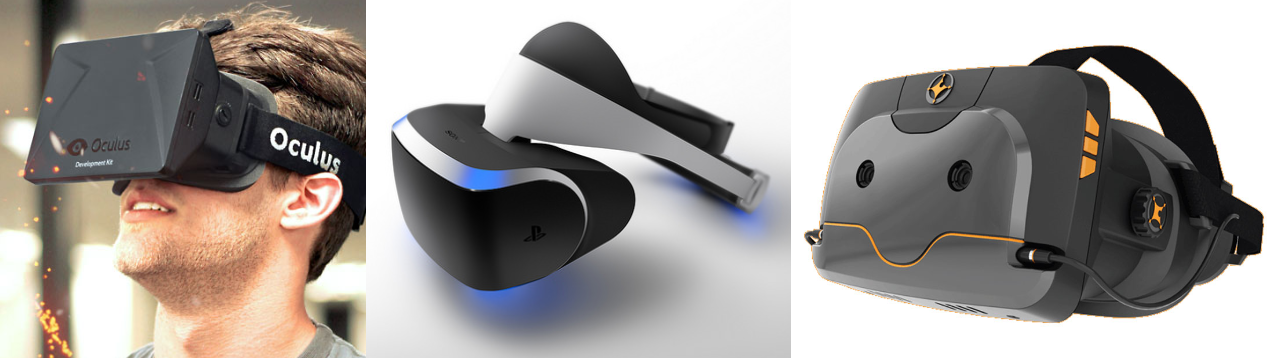
\includegraphics[width=1.0\textwidth]{images/hmds.png}
\caption{From left to right the Oculus Rift DK1, Sony's Project Morpheus, and True Player Gear's Toem. Images taken from \protect\cite{oculus-rift}, \protect\cite{project-morpheus}, and \protect\cite{true-player-gear}, respectively.}
\label{fig:hmds}
\end{figure}
 
Most of these technologies have remained outside of consumer reach, largely due to the large size and high cost of such systems, with the exception of HMDs, whose simplicity and compact design has led them to enjoy intermittent commercial availability for many years. A comprehensive discussion of commercially available HMDs is outside the scope of this paper, but it is worth noting that the recent release of OculusVR's ‘Oculus Rift' development kit to consumer markets has sparked a resurgence in interest in virtual reality for video games and other entertainment applications, leading to the announcement of several new consumer HMDs, including a consumer version of the Oculus Rift \cite{oculus-rift}, Sony's ‘Project Morpheus' \cite{project-morpheus}, and True Player Gear's ‘Totem' \cite{true-player-gear}. 

Priced at only a few hundred dollars, these HMDs put high resolution, wide field-of-view, immersive 3D display technology in the hands of everyday computer users, and the continuing advances of consumer graphics processing hardware gives them the ability to drive convincing 3D scenes onto these displays with commodity hardware. Furthermore, like 3D input devices, the similarity in function between these devices means their behavior can be captured abstractly by relatively simple input and output models. 
